\documentclass[11pt,addpoints,answers]{exam}

\usepackage[top=0.5in, left=0.75in, right=0.75in, bottom=.75in]{geometry}
\usepackage{amsmath,amsfonts,nicefrac, amssymb,amsxtra}
\usepackage{mathtools}
\usepackage{multicol}
\usepackage{pdfpages}
\usepackage{setspace}
\usepackage{enumitem}

%\usepackage{mathexam}
%\usepackage{latexsym}
%\usepackage[square, comma, sort&compress, numbers]{natbib}
%\usepackage{moresize}
%\usepackage{algpseudocode}
\usepackage{stmaryrd}
%\usepackage{enumitem}
%\renewcommand{\theenumi}{\alph{enumi}}
\usepackage{tabularx,ragged2e,booktabs,caption}
\usepackage{epstopdf}
\usepackage{epsfig}
\usepackage{setspace}
\usepackage{tikz,pgfplots}
\usetikzlibrary{arrows.meta}
\usetikzlibrary{arrows,decorations.markings}
\pgfplotsset{compat=1.14}
\usepgfplotslibrary{units}
\pgfplotsset{soldot/.style={color=black,only marks,mark=*}}
\pgfplotsset{holdot/.style={color=black,fill=white,only marks,mark=*}}
\usepackage{polynom}
\usepackage{enumerate}
\usepackage{graphicx,wrapfig,lipsum}
\allowdisplaybreaks


\usepackage[utf8]{inputenc}
\usetikzlibrary{decorations}
\usetikzlibrary{decorations.pathreplacing}
%\usepackage{fancyhdr}
\usepackage{array}
\usepackage{parskip}

\renewcommand{\arraystretch}{1.2}
\renewcommand\partlabel{(\thequestion.\arabic{partno})}

\newcommand{\emptybox}[2][\textwidth]{%
  \begingroup
  \setlength{\fboxsep}{-\fboxrule}%
  \noindent\framebox[#1]{\rule{0pt}{#2}}%
  \endgroup
}

\pgfplotsset{compat=1.14}


\begin{document}
\noindent {\Large Quiz, Fall Week 4 \hfill Name: \underline{\hspace{7cm}}}

\noindent {\normalsize {Points possible: \numpoints      \hfill Math 1050-90, Fall 2021, Due 9/21 at 11:59 p.m.}}

{\small \noindent \textbf{Rules/Suggestions:} Write with a dark pencil, so that your work is visible.  \textbf{You are graded on your work, not just answers. Even if you do calculations in your head or on scratch, show work if space is provided. } Write the final answer in the box.

Notes: You are on your honor for this to be your own work.  (You can ask for help on quiz material, but you should not ask for help on specific problems.) }
\begin{questions}

\question Compute the following, given $A=4-3i$ and $B=2+5i$. Show clear work. Simplify to write answers in the form, $a+bi$.
\begin{parts}\begin{multicols}{3}
\part[4] $B+A$
\part[4] $-7A$
\part[4] $AB$
\end{multicols}\end{parts}

\vspace{1in}
\begin{multicols}{3}
\begin{flushleft}
\fbox{%
\begin{minipage}{1.75in}
\hspace{1in}\\[4ex]
$B+A$ = \hrulefill\\[0.25ex]
\end{minipage}}
\end{flushleft}

\columnbreak

\begin{flushleft}
\fbox{%
\begin{minipage}{1.75in}
\hspace{1in}\\[4ex]
$-7A$ = \hrulefill\\[0.25ex]
\end{minipage}}
\end{flushleft}

\columnbreak

\begin{flushleft}
\fbox{%
\begin{minipage}{1.75in}
\hspace{1in}\\[4ex]
$AB$ = \hrulefill\\[0.25ex]
\end{minipage}}
\end{flushleft}
\end{multicols}
\vspace{0.2in}

\question Find the requested information for the function $P(x)=x^4+3x^3+5x^2+x-10$.  The graph of $P(x)$ is given below.

\begin{multicols}{2}
\scalebox{.9}{\begin{tikzpicture}
\begin{axis}[
every tick label/.append style={font=\small},
  axis lines=middle,
  grid=major,  major grid style={line width=.2pt,draw=white!50},   axis line style={latex-latex,line width=.8pt,black!100},
  xmin=-4,
  xmax=4,
  ymin=-20,
  ymax=20,
  xlabel=\small{$x$},
 ylabel=\small{$P(x)$},
  xtick={-4,-3,-2,-1,1,2,3,4,5},
  ytick={-10,0,10},
  yticklabels=\empty,
  xticklabels={-4,-3,-2,-1,1,2,3},
  tick style={thick}]
\addplot[<->,{Stealth[scale=1.4]}-{Stealth[scale=1.4]}, smooth, domain=-3:2, thick] {x^4+3*x^3+5*x^2+x-10};
\end{axis}
\end{tikzpicture}}

\columnbreak

\begin{parts}
\part[6] Find all the zeros of the function $P(x)$.
\end{parts}
\vspace{2in}
\begin{flushright}\fbox{%
\begin{minipage}{3in}
Zeroes:\\[3ex]
\end{minipage}}\end{flushright}

\end{multicols}

\begin{multicols}{2}
\begin{parts}
\part[6] Write the completely factored form of $P(x)$ into linear and irreducible quadratic factors.
\end{parts}

\columnbreak

\begin{flushright}\fbox{%
\begin{minipage}{3in}
Function:\\[3ex]
$P(x)= \ $\hrulefill\\[0.25ex]
\end{minipage}}\end{flushright}

\end{multicols}

  \vfill
\pagestyle{empty}
\hspace*{1in}{\Huge \textbf{Page 1}}

\newpage

\question[12] Solve the polynomial inequality $2x^2+16\geq x^2+8x+4$.  Write your answer in interval notation.  Show work for how you determine the answer.  (A sketch is highly recommended.)


\vspace*{1.5in}

\begin{flushright}

\fbox{%
\begin{minipage}{3in}
\hspace{1in}\\[1ex]
Answer: \\[3ex]
\end{minipage}}\end{flushright}

\question[12] Solve the polynomial inequality $(x-8)(x+6)(x-4)^2<0$.  Write your answer in interval notation  Show work for how you determine the answer.  (A sketch is highly recommended.)


\vspace*{1.5in}

\begin{flushright}

\fbox{%
\begin{minipage}{3in}
\hspace{1in}\\[1ex]
Answer: \\[3ex]
\end{minipage}}\end{flushright}

\question[20] The height $h$ in feet of a model rocket above the ground $t$ seconds after lift-off is given by $h(t)=-4t^2+72t$ for $0\leq t\leq 20$.  When is the rocket at least $288$ feet off the ground.  Show work for how you determine the answer.  (A sketch is highly recommended.)


\vspace*{1.5in}

\begin{flushright}

\fbox{%
\begin{minipage}{4in}
\hspace*{1in}\\[4ex]
\centering \underline{\hspace{2cm}} seconds $\leq t \leq$ \underline{\hspace{2cm}} seconds \\[2ex]
\hspace*{1in}
\end{minipage}}\end{flushright}



  \vfill
\pagestyle{empty}
\hspace*{2.75in}{\Huge \textbf{Page 2}}

\newpage

\setlength\columnsep{1cm}

\question Find the requested information for the function. Write asymptotes as equations and intercepts as ordered pairs.
$$ f(x)= \dfrac{3x^2+8x+4}{x^2-4}\\$$
\vspace{.1cm}
\begin{multicols}{2}

\begin{parts}
\part[8] Rewrite function with numerator and denominator factored:

\vspace*{1in}

\begin{flushright}

\fbox{%
\begin{minipage}{2.5 in}

$g(x)=$\\[6ex]
\end{minipage}}
\end{flushright}
\part[4] \hspace{1in}\\

\vspace*{-.3in}
\begin{flushright}
\fbox{%
\begin{minipage}{2.5 in}$x$-value of hole:\\[3ex]
\end{minipage}}
\fbox{%
\begin{minipage}{2.5 in}

vertical asymptote(s):\\[3ex]
\end{minipage}}
\end{flushright}



\part[4]\hspace{1in}\\

\vspace*{-.3in}
\begin{flushright}
\fbox{%
\begin{minipage}{2.5 in}

$x$-intercept(s):\\[3ex]
\end{minipage}}
\fbox{%
\begin{minipage}{2.5 in}

$y$-intercept:\\[3ex]
\end{minipage}}\end{flushright}


 \columnbreak


\part[6] \hspace{1in}\\

\vspace*{-.1in}
\begin{flushright}
\fbox{%
\begin{minipage}{2.5 in}

other asymptote:\\[3ex]
\end{minipage}}
\fbox{%
\begin{minipage}{2.5 in}

end behavior:\\
 As $x\rightarrow-\infty$, $f(x)\rightarrow$ \hrulefill\\

   As $x\rightarrow \infty$, $f(x)\rightarrow$ \hrulefill\\
\end{minipage}}
\fbox{%
\begin{minipage}{2.5 in}

Range: :\\[3ex]
\end{minipage}}
\end{flushright}


\vspace{.5cm}
\part[10] Sketch the
graph, carefully marking intercepts, asymptotes and holes.\\

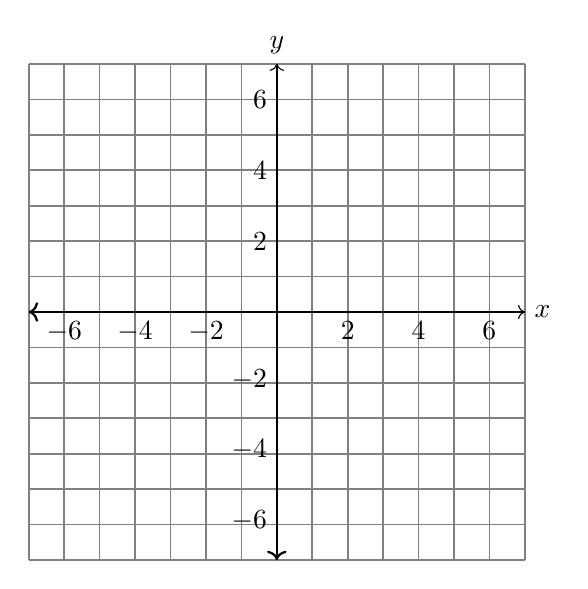
\begin{tikzpicture}[scale=.45]
\draw[help lines][semithick] (-7,-7) grid (7,7);
\draw[<-] [thick] (-7,0) -- (7,0) ;
\draw[<-] [thick] (0,-7) -- (0,7) ;
\foreach \x in {  -6, -4,  -2,  2,  4, 6 } \node[below] at (\x, 0) {$\x$};
\draw[->] (0, 0) -- (7, 0) node[right] {$x$};	% x-axis
\draw[->] (0, -7) -- (0, 7) node[above] {$y$};	% y-axis
\foreach \y/\ytext in { -5.9/-6, -3.9/-4, -1.9/-2,  2/2,4/4, 6/6} \node[left] at (0, \y) {$\ytext$};
\end{tikzpicture}
\end{parts}
\end{multicols}

\end{questions}

  \vfill
\pagestyle{empty}
\hspace*{5in}{\Huge \textbf{Page 3}}

\end{document}
